\documentclass{report}

\input{~/dev/latex/template/preamble.tex}
\input{~/dev/latex/template/macros.tex}

\title{\Huge{}}
\author{\huge{Nathan Warner}}
\date{\huge{}}
\pagestyle{fancy}
\fancyhf{}
\lhead{Warner \thepage}
\rhead{}
% \lhead{\leftmark}
\cfoot{\thepage}
%\setborder
% \usepackage[default]{sourcecodepro}
% \usepackage[T1]{fontenc}

\begin{document}
    % \maketitle
        \begin{titlepage}
       \begin{center}
           \vspace*{1cm}
    
           \textbf{Calculus 2} \\
           Chapter 5
    
           \vspace{0.5cm}
            
                
           \vspace{1.5cm}
    
           \textbf{Nathan Warner}
    
           \vfill
                
                
           \vspace{0.8cm}
         
           
\includegraphics[width=0.4\textwidth]{~/niu/seal.png}
                
           Computer Science \\
           Northern Illinois University\\
           October 27, 2023 \\
           United States\\
           
                
       \end{center}
    \end{titlepage}
    \tableofcontents
    \pagebreak \bigbreak \noindent
    \vspace{2in} \\
    \begin{Huge}
       \textbf{Sequences and Series} 
    \end{Huge}
    \bigbreak \noindent 
    \line(1,0){490}
    \bigbreak \noindent 

    \phantomsection
    \addcontentsline{toc}{section}{5.1 Sequences}
    \section*{5.1 Sequences}
    \bigbreak \noindent 
    \phantomsection
    \addcontentsline{toc}{subsection}{Terminology of Sequences}
    \subsection*{Terminology of Sequences}
    \bigbreak \noindent 
    To work with this new topic, we need some new terms and definitions. First, an infinite sequence is an ordered list of numbers of the form
    \begin{align*}
        a_{1},\ a_{2},\ a_{3},\ ...\ a_{n},\ ....
    .\end{align*}
    \bigbreak \noindent 
    Each of the numbers in the sequence is called a term. The symbol $n$ is called the index variable for the sequence. We use the notation
    \begin{align*}
        \{a_{n}\}_{n=1}^{\infty},\ \text{or simply}\ \{a_{n}\}
    .\end{align*}
    \bigbreak \noindent 
    to denote this sequence. A similar notation is used for sets, but a sequence is an ordered list, whereas a set is not ordered. Because a particular number $a_{n}$ exists for each positive integer $n$, we can also define a sequence as a function whose domain is the set of positive integers.
     \bigbreak \noindent 
    Let’s consider the infinite, ordered list
    \begin{align*}
        2,\ 4,\ 8,\ 16,\ 32,\ ...
    .\end{align*}
    \bigbreak \noindent 
    This is a sequence in which the first, second, and third terms are given by $a_1 = 2$, $a_2 = 4$, and $a_3 = 8$. You can probably see that the terms in this sequence have the following pattern:
    \begin{align*}
        a_{1} = 2^{1},\ a_{2} = 2^{2},\ a_{3} = 2^{3},\ a_{4}= 2^{4},\ \text{and}\ a_{5} = 2^{5}
    .\end{align*}
    \bigbreak \noindent 
    Assuming this pattern continues, we can write the $n^{th}$ term in the sequence by the explicit formula $a_n = 2^{n}$. Using this notation, we can write this sequence as
    \[
    \{2n\}_{n=1}^{\infty} \quad \text{or} \quad \{2n\}.
    \]
    \bigbreak \noindent 
    Alternatively, we can describe this sequence in a different way. Since each term is twice the previous term, this sequence can be defined recursively by expressing the $n^{th}$ term $a_n$ in terms of the previous term $a_{n-1}$. In particular, we can define this sequence as the sequence $\{a_n\}$ where $a_1=2$ and for all $n \geq 2$, each term $a_n$ is defined by the \textbf{recurrence relation} $a_n = 2a_{n-1}$.

    \pagebreak \bigbreak \noindent 
    \begin{definition}[Infinite Sequence]
        An infinite sequence $\{a_n\}$ is an ordered list of numbers of the form
        \[ a_1, a_2, \ldots, a_n, \ldots \]
        The subscript $n$ is called the index variable of the sequence. Each number $a_n$ is a term of the sequence. Sometimes sequences are defined by explicit formulas, in which case $a_n = f(n)$ for some function $f(n)$ defined over the positive integers. In other cases, sequences are defined by using a recurrence relation. In a recurrence relation, one term (or more) of the sequence is given explicitly, and subsequent terms are defined in terms of earlier terms in the sequence.


    \end{definition}

    \bigbreak \noindent 
    \nt{Note that the index does not have to start at $n=1$ but could start with other integers. For example, a sequence given by the explicit formula $a_{n}=f(n)$ could start at $n=0$,in which case the sequence would be
        \begin{align*}
            a_{0},\ a_{1},\ a_{2},\ ...
        .\end{align*}
    }
    \bigbreak \noindent 
    \begin{minipage}[t]{0.52\textwidth}
        Similarly, for a sequence defined by a recurrence relation, the term $a_0$ may be given explicitly, and the terms $a_n$ for $n \geq 1$ may be defined in terms of $a_{n-1}$. Since a sequence $\{a_n\}$ has exactly one value for each positive integer $n$, it can be described as a function whose domain is the set of positive integers. As a result, it makes sense to discuss the graph of a sequence. The graph of a sequence $\{a_n\}$ consists of all points $(n, a_n)$ for all positive integers $n$. Figure 5.2 shows the graph of $\{2n\}$.
    \end{minipage}
    \begin{minipage}[t]{0.47\textwidth}
         \begin{center}
            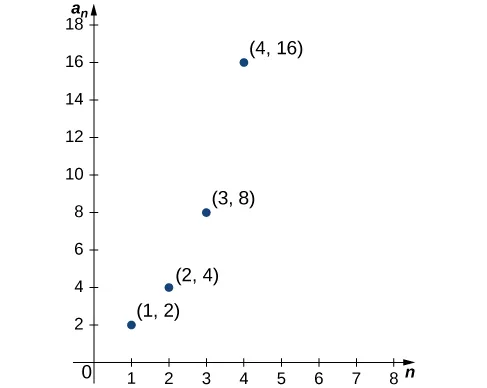
\includegraphics[scale=0.5]{./figures/mane6.png}
        \end{center}
        \begin{center}
            \textit{Figure 5.2}
        \end{center}
    \end{minipage}
    \bigbreak \noindent 

    





    



\end{document}
